\chapter{Discrete Geometry} \label{Ch7:CH}
\thispagestyle{empty}

We now put points in the plane and ask how many pairs of them can be at distance exactly $1$. In the language of \Cref{Ch2:Def:Unit_Distance_Graph}, this asks how many edges a subgraph of the unit distance graph on $n$ vertices can have, rather than how many colours it needs. Constructions give lower bounds; the upper bound will come from drawing graphs in the plane and counting how often their edges are forced to cross. The same counting then bounds how often points can lie on lines, and the chapter ends with lines in space and the points where three of them meet.

\section{The \protect\Erdos\ Unit Distance Problem}

The \Erdos\ Unit Distance Problem asks the following question:
\begin{center}
    \textbf{How many unit distances can there be amongst $n$ distinct points in $\R^2$?}
\end{center}

\subsection{Lower Bounds}

Some naïve constructions include making each point adjacent to four or six others by way of square/triangular tiling.
\begin{figure}[H]
    \centering
    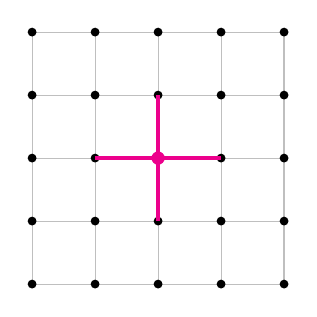
\begin{tikzpicture}[scale = 0.8]
        \draw[gray!50] (-2, -2) grid (2, 2);
        \foreach \x in {-2, ..., 2}{
            \foreach \y in {-2, ..., 2}{
                \fill[black] (\x, \y) circle (2pt);
            }
        }
        \foreach \ang in {0, 90, 180, 270}{
            \draw[very thick, magenta] (0, 0) -- (\ang:1);
        }
        \fill[magenta] (0, 0) circle (3pt);
    \end{tikzpicture}
    \qquad \qquad
    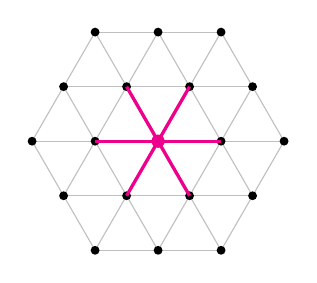
\begin{tikzpicture}[scale = 0.8]
        \foreach \j in {-2, ..., 2}{
            \foreach \i in {-2, ..., 2}{
                \pgfmathtruncatemacro{\hexdist}{max(abs(\i), abs(\j), abs(\i + \j))}
                \ifnum \hexdist < 3
                    \pgfmathsetmacro{\x}{\i + 0.5 * \j}
                    \pgfmathsetmacro{\y}{0.866 * \j}
                    \foreach \di/\dj/\ang in {1/0/0, 0/1/60, -1/1/120}{
                        \pgfmathtruncatemacro{\nextdist}{max(abs(\i + \di), abs(\j + \dj), abs(\i + \di + \j + \dj))}
                        \ifnum \nextdist < 3
                            \draw[gray!50, shift = {(\x, \y)}] (0, 0) -- (\ang:1);
                        \fi
                    }
                    \fill[black] (\x, \y) circle (2pt);
                \fi
            }
        }
        \foreach \ang in {0, 60, ..., 300}{
            \draw[very thick, magenta] (0, 0) -- (\ang:1);
        }
        \fill[magenta] (0, 0) circle (3pt);
    \end{tikzpicture}
\end{figure}

Another construction gives us even better numbers.

Take a square. Each vertex is connected to $2$ others. Translate it by one unit and connect it. Then each vertex is connected to $3$ others. Translate it by another unit and connect it again. Then each vertex is connected to $4$ others. Keep going. In this construction, you get $n \log(n)$ as your lower-bound.

More precisely, each translation is by a unit vector in a new direction, and the directions are chosen generically enough (a random choice works) that no two points ever coincide. The square is a $2$-dimensional cube, and each translation adds a dimension, so after $d - 2$ translations we have $n = 2^d$ points, each at unit distance from $d$ others. Each unit distance is counted from both of its ends, so there are at least
\begin{align*}
    \frac{nd}{2} = \frac{1}{2} n \log_2(n)
\end{align*}
of them.

\Erdos\ gave something even better: draw a grid with the points some distance $\frac{1}{R}$ apart, where $R$ has the property that $R^2 = a^2 + b^2$ in many ways. The point is that this looks like the following:
\begin{figure}[H]
    \centering
    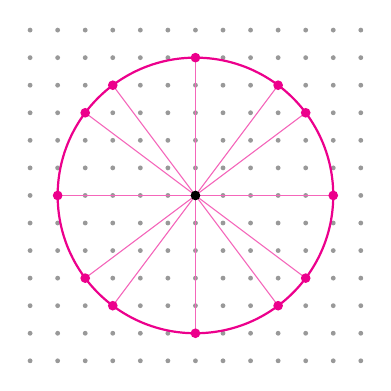
\begin{tikzpicture}[scale = 0.35]
        \foreach \x in {-6, ..., 6}{
            \foreach \y in {-6, ..., 6}{
                \fill[black!40] (\x, \y) circle (2.5pt);
            }
        }
        \draw[thick, magenta] (0, 0) circle (5);
        \foreach \x/\y in {5/0, 4/3, 3/4, 0/5, -3/4, -4/3, -5/0, -4/-3, -3/-4, 0/-5, 3/-4, 4/-3}{
            \draw[magenta!60] (0, 0) -- (\x, \y);
            \fill[magenta] (\x, \y) circle (5pt);
        }
        \fill[black] (0, 0) circle (5pt);
    \end{tikzpicture}
\end{figure}
Here $R = 5$, and $25 = 0^2 + 5^2 = 3^2 + 4^2 = 4^2 + 3^2$ puts $12$ grid points on the circle of radius $R$ grid units, ie, at unit distance from the centre.

We can then do some very nice algebraic number theory involving $\Z[i]$ to get
\begin{align*}
    n^{1 + \frac{c}{\log\of{\log(n)}}}
\end{align*}

\Erdos\ conjectured that the maximum you could get to is $n^{1 + o(1)}$. OpenAI disproved this by finding an $n^{1 + \delta}$ construction for some $\delta > 0$.

% [CORRECTED] was: "an upper-bound: $n^{\frac{4}{3}}$" --- the Spencer--Szemer\'{e}di--Trotter bound has a constant
% in it, and the best known one is above $1$; with constant $1$ it is not a theorem.
We will not get into the lower-bounds here, but we will show an upper-bound: $\BigO{n^{\frac{4}{3}}}$. The tool for it is drawing graphs in the plane.

\subsection{Planar Graphs}

We also make a distinction between plane and planar graphs: planar graphs are abstract graphs with drawings in the plane, and plane graphs are the actual drawings themselves. More formally, we define the following.

\begin{boxdefinition}[Planar Graph]
    A graph $G$ is \textbf{planar} if it has an \textbf{embedding} in the plane: an injective map sending each vertex to a point of $\R^2$ and each edge $\set{u, v}$ to a curve joining the images of $u$ and $v$, such that no curve passes through the image of any other vertex and no two curves meet except at a common endpoint.
\end{boxdefinition}

The picture itself is then the following.

\begin{boxdefinition}[Plane Graph]
    A \textbf{plane graph} is the image of an embedding of a planar graph: the points and curves in $\R^2$ themselves. Its \textbf{faces} are the connected components of what remains of $\R^2$ once the plane graph is removed.
\end{boxdefinition}

Not all graphs are planar.

\begin{boxnexample}[Non-planar graphs]
    $K_5$, $K_{100}$, any $K_n$ for $n \geq 5$.
    \begin{figure}[H]
        \centering
        \begin{tikzpicture}
            \completegraph{5}
        \end{tikzpicture}
    \end{figure}
\end{boxnexample}

The reason graphs fail to be planar is that too many of their edges cross.

We follow the lecture's letters for the sizes of a graph.

\begin{boxlnotation}
    For the rest of this section, a graph $G$ has $n$ vertices and $m$ edges, and a plane graph has $f$ faces. Where several graphs are in play, we write $n(H)$ and $m(H)$ for the numbers of vertices and edges of $H$.
\end{boxlnotation}

(Connected) plane graphs satisfy Euler's Formula: $n - m + f = 2$. We can prove this using induction on $m$ and some handwaving (one should say ``visual intuition''), but to actually do this rigorously takes a lot of machinery (eg. the Jordan Curve Theorem).

\begin{boxtheorem}[Euler's Formula]
    For a connected plane graph with $n$ vertices, $m$ edges and $f$ faces,
    \begin{align*}
        n - m + f = 2
    \end{align*}
\end{boxtheorem}
\begin{proof}
    Induction on $m$. \sorry % [CLAUDE] don't fill this in, it's an exercise for me to do later.
\end{proof}

% [CORRECTED] was: "in any plane graph" --- a single edge, or a path with two edges, is a plane graph with one face
% incident with fewer than $3$ edges, and a loop or a pair of parallel edges bounds such a face too. The
% proposition below, which is what uses the first item, assumes this (and connectedness besides).
Notice that in any simple plane graph with at least $3$ edges, we \textit{must} have
\begin{itemize}
    \item Every face is incident with $\geq 3$ edges
    \item Every edge is incident with $\leq 2$ faces
\end{itemize}

This gives us an important inequality.

\begin{boxproposition} \label{Ch7:Prop:Planar_Edge_Bound}
    For any connected simple plane graph with $n$ vertices, $m$ edges and $f$ faces, if $m \geq 3$, then
    \begin{align*}
        m \leq 3n - 6
    \end{align*}
\end{boxproposition}
\begin{proof}
    Count edge-face incidences. By above,
    \begin{align*}
        3f \leq \sum_{F \text{ a face}} \#\!\set{\text{edges $F$ is incident with}} = \sum_{E \text{ an edge}} \#\!\set{\text{faces $E$ is incident with}} \leq 2m
    \end{align*}
    Thus, we get the equivalent inequalities
    \begin{align*}
        3f \leq 2m \qquad \iff  \qquad f \leq \frac{2m}{3}
    \end{align*}
    Combining with Euler's formula, we get
    \begin{align*}
        2
        = n - m + f
        \leq n - m + \frac{2m}{3}
        = n - \frac{m}{3}
    \end{align*}
    Rearranging gives us the desired inequality.
\end{proof}

\subsection{Crossing Numbers}

A graph that is not planar can still be drawn in the plane, and we can ask how few crossings it needs.

\begin{boxdefinition}[Crossing Number]
    For every finite simple graph $G$, define the \textbf{crossing number}, denoted $\pcr{G}$, to be the minimum number of crossings between edges, taken over all drawings of $G$ in the plane. Ie, define
    \begin{align*}
        \pcr{G} = \min_{\text{drawings of $G$ in the plane}} \#\!\set{\text{crossings between edges}}
    \end{align*}
\end{boxdefinition}

We might expect $\pcr{K_n} = \BigO{\parenth{\#\text{edges}}^2} = \BigO{n^4}$.

\Cref{Ch7:Prop:Planar_Edge_Bound} gives us a first lower bound.

\begin{boxlemma} \label{Ch7:Lemma:Crossing_Edge_Bound}
    If $G$ is simple, then $\pcr{G} \geq m - 3n$.
\end{boxlemma}
% [FILLED] proof supplied here; the lecture stated the lemma without proving it
\begin{proof}
    First, every simple plane graph $H$ has $m(H) \leq 3n(H)$. Indeed, each connected component of $H$ is a connected simple plane graph in its own right: a component with $n_i$ vertices and $m_i \geq 3$ edges has $m_i \leq 3n_i - 6 \leq 3n_i$ by \Cref{Ch7:Prop:Planar_Edge_Bound}, and one with $m_i \leq 2$ edges has $m_i \leq 3n_i$ since $n_i \geq 1$. Summing over the components gives $m(H) \leq 3n(H)$.

    Now take a drawing of $G$ with exactly $\pcr{G}$ crossings, and for each crossing delete one of the two edges involved. We have deleted at most $\pcr{G}$ edges, and what remains is a drawing with no crossings at all, ie, a simple plane graph on the same $n$ vertices with at least $m - \pcr{G}$ edges. Thus $m - \pcr{G} \leq 3n$, which rearranges to $\pcr{G} \geq m - 3n$.
\end{proof}

Consider the case $G = K_n$. So $m = \binom{n}{2}$. The above inequality gives us
\begin{align*}
    \pcr{K_n} \geq \binom{n}{2} - 3n
\end{align*}
But we can probably do better than this: we'd at least expect each edge to cross each other edge or something, so we might think $\pcr{K_n} = \Omega\of{n^4}$.

\subsection{The Crossing Lemma}

Probabilistic methods to the rescue!

\begin{boxlnotation}
    Given a graph $G$ and $p \in [0, 1]$, define $G_p$ to be the graph that retains vertices of $G$ independently with probability $p$ (ie, that deletes vertices of $G$ independently with probability $1 - p$). Define random variables $n_p$ and $m_p$, respectively denoting the number of vertices and edges in $G_p$. Denote by $n$ and $m$ the number of vertices and edges respectively of $G$.
\end{boxlnotation}

We actually want to think of $G_p$ as the space of all subgraphs of $G$, with the power sigma algebra, with each singleton (ie, the probability of each subgraph being realised) having probability determined by $p$.

\begin{boxlemma} \label{Ch7:Lemma:Gp_Expectations}
    $\E\of{n_p} = p \cdot n$ and $\E\of{m_p} = p^2 \cdot m$.
\end{boxlemma}
\begin{proof}[Proof sketch]
    $\E\of{n_p} = p \cdot n$ is clear. To compute $\E\of{m_p}$, define indicator random variables $\xi_e$ for each edge $e$, so that $m_p$ is the sum over all edges $e$ of the $\xi_e$. Then apply linearity of expectation.
\end{proof}

We can relate $\pcr{G_p}$ with $\pcr{G}$.

\begin{boxlemma} \label{Ch7:Lemma:Gp_Crossings}
    $\E\of{\pcr{G_p}} \leq p^4 \cdot \pcr{G}$
\end{boxlemma}
\begin{proof}
    \sorry
    % Hint: fix a drawing of $G$ with exactly $\pcr{G}$ crossings, and draw each outcome of $G_p$ by erasing the deleted vertices and every edge at them. This is a drawing of $G_p$, so $\pcr{G_p}$ is at most the number of crossings that survive into it. When does a crossing survive, and with what probability? Then take expectations.
    % Second hint, for the probability: you want the two edges at a crossing to have four distinct endpoints between them. In a drawing with the fewest crossings, two edges that share an endpoint never cross --- if they did, swapping their two pieces between the shared endpoint and the crossing point, and pulling them slightly apart, would give a drawing with fewer crossings.
\end{proof}

If we can then find a tighter lower-bound for $\pcr{G_p}$, we can get a tighter lower-bound for $\pcr{G}$. If we then optimise it by finding the $p$ that makes it tightest, we can actually do a bit better than what we've done so far.

This is the content of the following theorem.

% [FILLED] statement and proof written up from the blackboard photographs supplied with the post-lecture pass of 2026-10-27; the \sorry in the proof is left as an exercise, with a hint
\begin{boxtheorem}[The Crossing Lemma] \label{Ch7:Thm:Crossing_Lemma}
    If $G$ is a simple graph with $n$ vertices and $m \geq 4n$ edges, then
    \begin{align*}
        \pcr{G} \geq \frac{m^3}{64n^2}
    \end{align*}
\end{boxtheorem}
\begin{proof}
    We claim that for every $p \in (0, 1]$,
    \begin{align*}
        p^4 \pcr{G} \geq p^2 m - 3pn
    \end{align*}
    \sorry
    % Hint: every outcome of $G_p$ is a simple graph, so \Cref{Ch7:Lemma:Crossing_Edge_Bound} applies to it. That gives an inequality between three random variables; take expectations of both sides, and bring in \Cref{Ch7:Lemma:Gp_Expectations,Ch7:Lemma:Gp_Crossings}.

    Dividing through by $p^4$, we get
    \begin{align*}
        \pcr{G} \geq \frac{m}{p^2} - \frac{3n}{p^3}
    \end{align*}
    for every $p \in (0, 1]$, and we are free to choose $p$. We take $p = \frac{4n}{m}$, which is a probability precisely because $m \geq 4n$. (This is not quite the $p$ that maximises the right-hand side, but it makes the constant come out cleanly.) Substituting,
    \begin{align*}
        \pcr{G}
        \geq \frac{m^3}{16n^2} - \frac{3m^3}{64n^2}
        = \frac{m^3}{64n^2}
    \end{align*}
\end{proof}

In particular, once $n \geq 9$ we have $\binom{n}{2} \geq 4n$, so
\begin{align*}
    \pcr{K_n}
    \geq \frac{1}{64n^2} \binom{n}{2}^3
    = \frac{n\parenth{n - 1}^3}{512}
    = \Omega\of{n^4}
\end{align*}

\subsection{A Unit-Distance Upper-Bound}

% Written up from the blackboard photographs supplied with the post-lecture pass of 2026-10-27; the three parts of the lemma are left \sorry as exercises, with hints
We can now give the upper-bound we promised. Throughout this subsection, fix a set $X$ of $n$ points in $\R^2$, with $m$ unit distances among them. For each $p \in X$, let $C_p$ be the unit circle centred at $p$, and let $\deg(p)$ be the number of points of $X$ on $C_p$: its degree in the unit distance graph on $X$. Each unit distance is counted at both of its ends, so
\begin{align*}
    2m = \sum_{p \in X} \deg(p)
\end{align*}

The idea is to draw a graph on $X$ using these circles, and to play the crossing lemma off against the fact that circles cannot cross each other very often. Discard every circle $C_p$ with $\deg(p) \leq 2$. Each remaining circle passes through at least $3$ points of $X$, which cut it into $\deg(p)$ arcs. Let $D$ be the drawing whose vertices are the points of $X$ and whose edges are all of these arcs, from all of the remaining circles.
\begin{figure}[H]
    \centering
    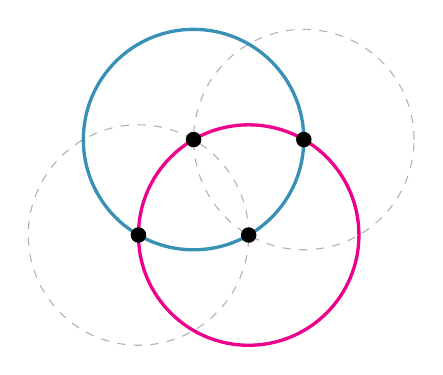
\begin{tikzpicture}[scale = 1.4]
        \draw[gray!60, dashed] (0, 0) circle (1);
        \draw[gray!60, dashed] (1.5, 0.866) circle (1);
        \draw[very thick, magenta] (1, 0) circle (1);
        \draw[very thick, cyan!70!black] (0.5, 0.866) circle (1);
        \foreach \x/\y in {0/0, 1/0, 0.5/0.866, 1.5/0.866}{
            \fill[black] (\x, \y) circle (2pt);
        }
    \end{tikzpicture}
\end{figure}
Here $n = 4$ and $m = 5$. The two dashed circles pass through only two points each and are discarded; each solid circle is cut into three arcs, so $D$ has $6$ edges, and the two long arcs both join the bottom-left point to the top-right one.

That last observation is the catch: two points can be joined by more than one arc, so $D$ is a drawing of a multigraph rather than a graph. But not by much.

\begin{boxlemma} \label{Ch7:Lemma:Circle_Drawing} \hfill
    \begin{enumerate}[label = (\arabic*)]
        \item $D$ has at least $2m - 2n$ edges.
        \item No two vertices of $D$ are joined by more than $2$ edges.
        \item There are at most $n^2$ crossings between edges of $D$.
    \end{enumerate}
\end{boxlemma}
\begin{proof} \hfill
    \begin{description}
        \item[\underline{(1).}] \sorry
        % Hint: how many edges does each remaining circle contribute? Compare the total with $2m = \sum_p \deg(p)$: how much can discarding the circles with $\deg(p) \leq 2$ have cost?
        \item[\underline{(2).}] \sorry
        % Hint: if an arc of $C_p$ joins $u$ and $v$, then $p$ is at distance $1$ from both of them. How many such points $p$ are there? And how many of the arcs of a single circle through at least $3$ points can join $u$ to $v$?
        \item[\underline{(3).}] \sorry
        % Hint: two arcs of the same circle never cross. Two different circles meet in at most $2$ points, and at each of these at most one arc of each circle passes through. Now count pairs of circles.
    \end{description}
\end{proof}

Now we just have to throw away the duplicate edges and apply the crossing lemma.

\begin{boxtheorem} \label{Ch7:Thm:Unit_Distance_Upper_Bound}
    Among any $n$ points in $\R^2$, there are at most $5n^{\frac{4}{3}}$ unit distances.
\end{boxtheorem}
\begin{proof}
    Let $\overline{D}$ be what remains of $D$ when we keep just one edge between each pair of vertices that $D$ joins. By \Cref{Ch7:Lemma:Circle_Drawing} (2) and then (1), $\overline{D}$ has at least half as many edges as $D$, so at least $m - n$ of them. It is a drawing of a simple graph $\overline{G}$ on $n$ vertices, and its crossings are among those of $D$, so by \Cref{Ch7:Lemma:Circle_Drawing} (3),
    \begin{align*}
        \pcr{\overline{G}} \leq n^2
    \end{align*}
    If $m - n < 4n$, then $m < 5n \leq 5n^{\frac{4}{3}}$ and we are done. Otherwise $\overline{G}$ has at least $m - n \geq 4n$ edges, and \Cref{Ch7:Thm:Crossing_Lemma} gives
    \begin{align*}
        n^2 \geq \pcr{\overline{G}} \geq \frac{\parenth{m - n}^3}{64n^2}
    \end{align*}
    Thus $\parenth{m - n}^3 \leq 64n^4$, ie, $m - n \leq 4n^{\frac{4}{3}}$, and $m \leq 4n^{\frac{4}{3}} + n \leq 5n^{\frac{4}{3}}$.
\end{proof}

\section{Point--Line Incidences}

The crossing lemma also bounds how often points of the plane can lie on lines, and the bound in turn says something about sums and products of integers.

\subsection{The Szemer\'{e}di--Trotter Theorem}

Given finite sets $\mathcal{L}$ of lines and $P$ of points in $\R^2$, define
\begin{align*}
    I\of{\mathcal{L}, P}
    := \#\!\set{\text{point-line incidences}}
    = \#\!\setst{\parenth{\ell, p} \in \mathcal{L} \times P}{p \in \ell}
\end{align*}

It turns out that we can say how large this can be, up to a constant.

\begin{boxtheorem}[Szemer\'{e}di--Trotter] \label{Ch7:Thm:Szemeredi_Trotter}
    $I\of{\mathcal{L}, P} = \BigO{\abs{\mathcal{L}}^{\frac{2}{3}} \abs{P}^{\frac{2}{3}} + \abs{\mathcal{L}} + \abs{P}}$
\end{boxtheorem}
\begin{proof}
    Given an $\mathcal{L},P$ system, consider the graph drawing $D$ whose vertices are the points in $P$ and whose edges are intervals of lines in $\mathcal{L}$ with endpoints in $P$, with no interior points in $P$.

    % [CORRECTED] was: "Let $P'$ with $\abs{P'} \leq \abs{P} + 2 \abs{\mathcal{L}}$ be an expected set of points such that every line has $\geq 2$ points." --- with up to $2\abs{\mathcal{L}}$ added points the argument below gives a term of order $\abs{\mathcal{L}}^{4/3}$, which the bound cannot absorb when $\abs{\mathcal{L}}$ is much larger than $\abs{P}$. The sentence now carries out the reduction of the author's own comment, which stood here: "I need to assume here that each line has at least 2 points. Then I argue and get my bound. Now in the general case, what I do is, I remove all lines with just one point, I get my upper-bound, then I add them back, which adds at most |L|, which gets subsumed into the |L| term of our big O."
    We first assume that every line of $\mathcal{L}$ contains at least $2$ points of $P$. In the general case, we remove the lines containing fewer than $2$ points of $P$, get our upper-bound for the lines that remain, and then add them back, which adds at most $\abs{\mathcal{L}}$ incidences; these are absorbed into the $\abs{\mathcal{L}}$ term of the bound.

    Let $n = \abs{P}$ be the number of vertices. How many edges do I have? I should have
    \begin{align*}
        m
        = I\of{\mathcal{L}, P} - \abs{\mathcal{L}}
        = \sum_{\ell \in \mathcal{L}} \parenth{\#\!\setst{p \in P}{p \in \ell} - 1}
    \end{align*}
    % [CORRECTED] was: "$n \leq 4m$, ie, $\abs{P'} \leq 4\parenth{I\of{\mathcal{L}, P} - \abs{P}}$" --- the crossing lemma needs $m \geq 4n$, and $m = I\of{\mathcal{L}, P} - \abs{\mathcal{L}}$
    If we have $4n \leq m$, ie,
    \begin{align*}
        4\abs{P} \leq I\of{\mathcal{L}, P} - \abs{\mathcal{L}}
    \end{align*}
    % [CORRECTED] was: "$\pcr{D} \leq \frac{\parenth{I\of{\mathcal{L}, P} - \abs{P}}^3}{64 \abs{P'}^2}$" --- the crossing lemma bounds $\pcr{D}$ from below, by $\frac{m^3}{64n^2}$
    then we can apply \Cref{Ch7:Thm:Crossing_Lemma} to conclude that
    \begin{align*}
        \pcr{D} \geq \frac{\parenth{I\of{\mathcal{L}, P} - \abs{\mathcal{L}}}^3}{64 \abs{P}^2}
    \end{align*}
    \sorry
    % Hint (from the blackboard): bound $\pcr{D}$ from above by $\abs{\mathcal{L}}^2$ --- where can two edges of $D$ cross, and how often can two lines meet? Comparing the two bounds on $\pcr{D}$ bounds $m$, and so $I\of{\mathcal{L}, P}$; the case $m < 4n$ needs a line of its own.
\end{proof}

\subsection{Sums and Products}

Fix some $A \ssq \Z$. Define
\begin{align*}
    A + A &:= \setst{a + b}{a, b \in A} \\
    A \cdot A &:= \setst{a \cdot b}{a, b \in A}
\end{align*}

Is there a set $A$ for which both $A + A$ and $A \cdot A$ are small?

To answer this, we turn it into an incidence problem. Define
\begin{align*}
    P := \parenth{A + A} \times \parenth{A \cdot A}
    = \setst{(x, y) \in \Z \times \Z}{x \in A + A, \, y \in A \cdot A}
\end{align*}
For example, when $A = \set{1, 2, 3}$, we have $A + A = \set{2, \ldots, 6}$ and $A \cdot A = \set{1, 2, 3, 4, 6, 9}$, and $P$ looks like this.
\begin{figure}[H]
    \centering
    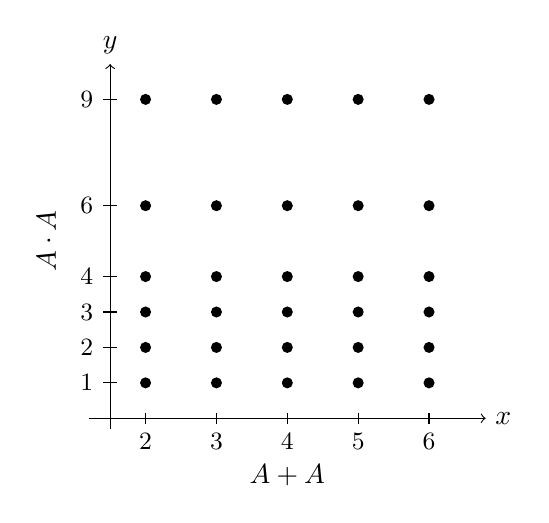
\begin{tikzpicture}[x = 0.9cm, y = 0.45cm]
        \draw[->] (1.2, 0) -- (6.8, 0) node[right] {$x$};
        \draw[->] (1.5, -0.3) -- (1.5, 10) node[above] {$y$};
        \foreach \x in {2, ..., 6}{
            \draw (\x, 0.15) -- (\x, -0.15) node[below] {\small $\x$};
        }
        \foreach \y in {1, 2, 3, 4, 6, 9}{
            \draw (1.6, \y) -- (1.4, \y) node[left] {\small $\y$};
            \foreach \x in {2, ..., 6}{
                \fill[black] (\x, \y) circle (2pt);
            }
        }
        \node at (4, -1.6) {$A + A$};
        \node[rotate = 90] at (0.6, 5) {$A \cdot A$};
    \end{tikzpicture}
\end{figure}

The incidence bound answers our question: $A + A$ and $A \cdot A$ cannot both be small.

% [FILLED] statement written up from the blackboard photographs supplied on 2026-10-27; the proof is left to the author, with a hint
\begin{boxtheorem} \label{Ch7:Thm:Sum_Product}
    There is a constant $c > 0$ such that for every finite $A \ssq \Z$,
    \begin{align*}
        \abs{A + A} \abs{A \cdot A} \geq c \abs{A}^{\frac{5}{2}}
    \end{align*}
    In particular, $\max\set{\abs{A + A}, \abs{A \cdot A}} \geq \sqrt{c} \abs{A}^{\frac{5}{4}}$.
\end{boxtheorem}
\begin{proof}
    \sorry
    % Hint (from the blackboard): use $P$ as above, so that $\abs{P} = \abs{A + A}\abs{A \cdot A}$, and let $\mathcal{L}$ be the $\abs{A}^2$ lines $y = a\parenth{x - a'}$ for $a, a' \in A$ (assume $0 \notin A$). Each of them passes through $\abs{A}$ points of $P$ --- try $x = a' + b$ for $b \in A$ --- so $I\of{\mathcal{L}, P} \geq \abs{A}^3$. Now compare this with \Cref{Ch7:Thm:Szemeredi_Trotter}, one term of its bound at a time.
\end{proof}

\section{Lines in $\R^3$}

\begin{boxdefinition}[Joint]
    A \textbf{joint} in $\R^3$ is an intersection point of $3$ non-coplanar lines.
\end{boxdefinition}

In other words, any point at which three lines that do not share a plane in common meet is called a joint.

We ask ourselves the following question: how many joints can a collection of $L$ lines have?

Let's denote the greatest such number $J(L)$.

Here's one construction: just an $n \times n \times n$ grid. This gives you $3n^2$ lines and $n^3$ joints.

\begin{figure}[H]
    \centering
    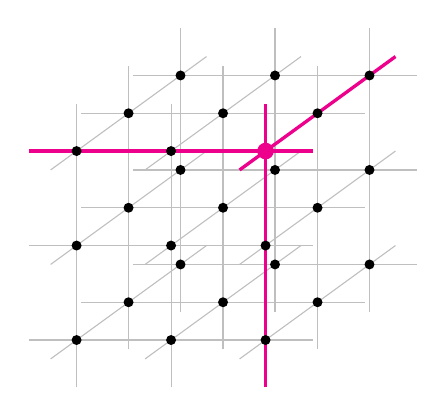
\begin{tikzpicture}[x = {(1cm, 0cm)}, y = {(0.55cm, 0.4cm)}, z = {(0cm, 1cm)}, scale = 1.2]
        \foreach \a in {0, 1, 2}{
            \foreach \b in {0, 1, 2}{
                \draw[gray!50] (-0.5, \a, \b) -- (2.5, \a, \b);
                \draw[gray!50] (\a, -0.5, \b) -- (\a, 2.5, \b);
                \draw[gray!50] (\a, \b, -0.5) -- (\a, \b, 2.5);
            }
        }
        \draw[very thick, magenta] (-0.5, 0, 2) -- (2.5, 0, 2);
        \draw[very thick, magenta] (2, -0.5, 2) -- (2, 2.5, 2);
        \draw[very thick, magenta] (2, 0, -0.5) -- (2, 0, 2.5);
        \foreach \a in {0, 1, 2}{
            \foreach \b in {0, 1, 2}{
                \foreach \c in {0, 1, 2}{
                    \fill[black] (\a, \b, \c) circle (1.5pt);
                }
            }
        }
        \fill[magenta] (2, 0, 2) circle (2.5pt);
    \end{tikzpicture}
\end{figure}
The case $n = 3$ is drawn above, with the three lines through one of the joints highlighted. Every point of the grid is a joint, and every line of the grid is parallel to one of the axes and passes through $n$ of them.

\begin{boxlemma}
    In any collection of lines with $J$ joints, some line is in $\leq 3J^{\frac{1}{3}}$ joints.
\end{boxlemma}
\begin{proof}
    \sorry
\end{proof}

Assuming the lemma, we notice that
\begin{align*}
    J(L)
    &\leq J(L - 1) + 3J(L)^{\frac{1}{3}} \\
    &\leq J(L - 2) + 3 \cdot 2 \cdot J(L)^{\frac{1}{3}} \\
    &\leq J(L - 3) \cdots \\
    &\leq 3 \cdot L \cdot J(L)^{\frac{1}{3}}
\end{align*}
The first inequality comes from taking $L$ lines with $J(L)$ joints and deleting a line that, by the lemma, is in at most $3J(L)^{\frac{1}{3}}$ of them. Every other joint is still a joint of the remaining $L - 1$ lines, so $J(L) - 3J(L)^{\frac{1}{3}} \leq J(L - 1)$. The same argument gives $J(L - 1) \leq J(L - 2) + 3J(L - 1)^{\frac{1}{3}}$, and $J(L - 1) \leq J(L)$, since adding a line to a collection destroys none of its joints; this is the second line. Carrying on down to $J(0) = 0$, each of the $L$ lines we delete costs at most $3J(L)^{\frac{1}{3}}$ joints, which is the last line. Dividing it by $J(L)^{\frac{1}{3}}$ gives $J(L)^{\frac{2}{3}} \leq 3L$, ie,
\begin{align*}
    J(L) \leq \parenth{3L}^{\frac{3}{2}} = \BigO{L^{\frac{3}{2}}}
\end{align*}
So the grid is optimal up to a constant factor: it has $L = 3n^2$ lines and $n^3 = \parenth{\frac{L}{3}}^{\frac{3}{2}}$ joints.

Let's now take a detour into the world of polynomials.

Our notation for this course isn't amazing. Let $\F$ be a field.

\begin{boxnotation}
    $\poly_D\of{\F^n}$ denotes the set
    \begin{align*}
        \setst{p \in \F\!\brac{x_1, \ldots, x_n}}{\deg_{\tot}\of{p} \leq D}
    \end{align*}
    where $\deg_{\tot}$ denotes the total degree of the polynomial.
\end{boxnotation}

The monomials form a basis of this space. By a stars and bars argument, we can show that the number of monomials is $\binom{D + n}{n}$. So this is the dimension of this space.

% [CORRECTED] was: "$\abs{S} \leq \dim\of{\poly_D\of{\F^n}}$, there is some $p$", and "the inequality $\abs{S} \leq \parenth{\text{dimension of space}}$" below --- $p = 0$ always vanishes, and at equality the kernel can be $0$ (eg, $n = 1$ and $D + 1$ distinct points), so the inequality has to be strict
Observe the following: if $S \ssq \F^n$ is such that $\abs{S} < \dim\of{\poly_D\of{\F^n}}$, there is some nonzero $p \in \poly_D\of{\F^n}$ that vanishes on $S$. The proof is simple: consider the evaluation map
\begin{align*}
    \ev : \poly_D\of{\F^n} \to \F^{S} : p \mapsto \parenth{p(s)}_{s \in S}
\end{align*}
Rank-nullity\footnote{Tarun would be so proud!} and the inequality $\abs{S} < \parenth{\text{dimension of space}}$ tells us the dimension of the kernel is positive, which gives us some $p$ as desired.

